\section{Module 1. MRI reconstruction}

Classical least squares estimation provides only the minimization of data error, which is an invalid solution. Conventionally, the LSE solution has a huge norm and thus it is a valueless outcome of a~reconstruction procedure. To this end, we introduced basic Tikhonov regularization method that seem to partially overcome the problem. However, we firstly implemented LSE approach for later usage of the results obtained with this procedure in restoration of the images from a~`nearby' well-posed problem (regularization). For Tikhonov regularization, additional quadratic penalty term allows controlling the norm of the solution, which benefits in introduction of smoothness prior to estimated solution. 

Firstly, we checked the data dimension that we load to the programme, as we could receive data starting from 3D to 5D. The implementation works for single slice structural and diffusion data (from many gradients) as well as for a whole set of brain slices. First two dimensions, provides information about data resolution i.e. $128\times 256$, which means that the images where subsampled with factor $r=2$. In case of structural data, the third dimension would be the number of slices (then, the forth is number of coils images) or simply number of coils images. For diffusion data, in 5D case the third dimension stands for number of slices, the forth - number of diffusion gradients and the fifth - number of coils images. The third dimension can be equal to one, so we get 4D data i.e. diffusion data for one slice. We also tested whether input dataset contains matrices with sensitivity maps profiles of a proper size, corresponding to maximal dimension of an image i.e. $256\times 256\times 8$, for case of images acquired with $8$ coils. Furthermore, the input files should also contain subsampling factor $r$ and number of coils $L$, if not, they can be calculated having the dataset's dimensional information.
 
Secondly, we performed 2D inverse Fourier Transform (2D IFT) on each of the dataset image, to transform them from \textbf{k}-space to \textbf{x}-space. This stage of an algorithm is presented in Fig. \ref{rys:subsampled}.  

\begin{figure}[h!]
\centering
  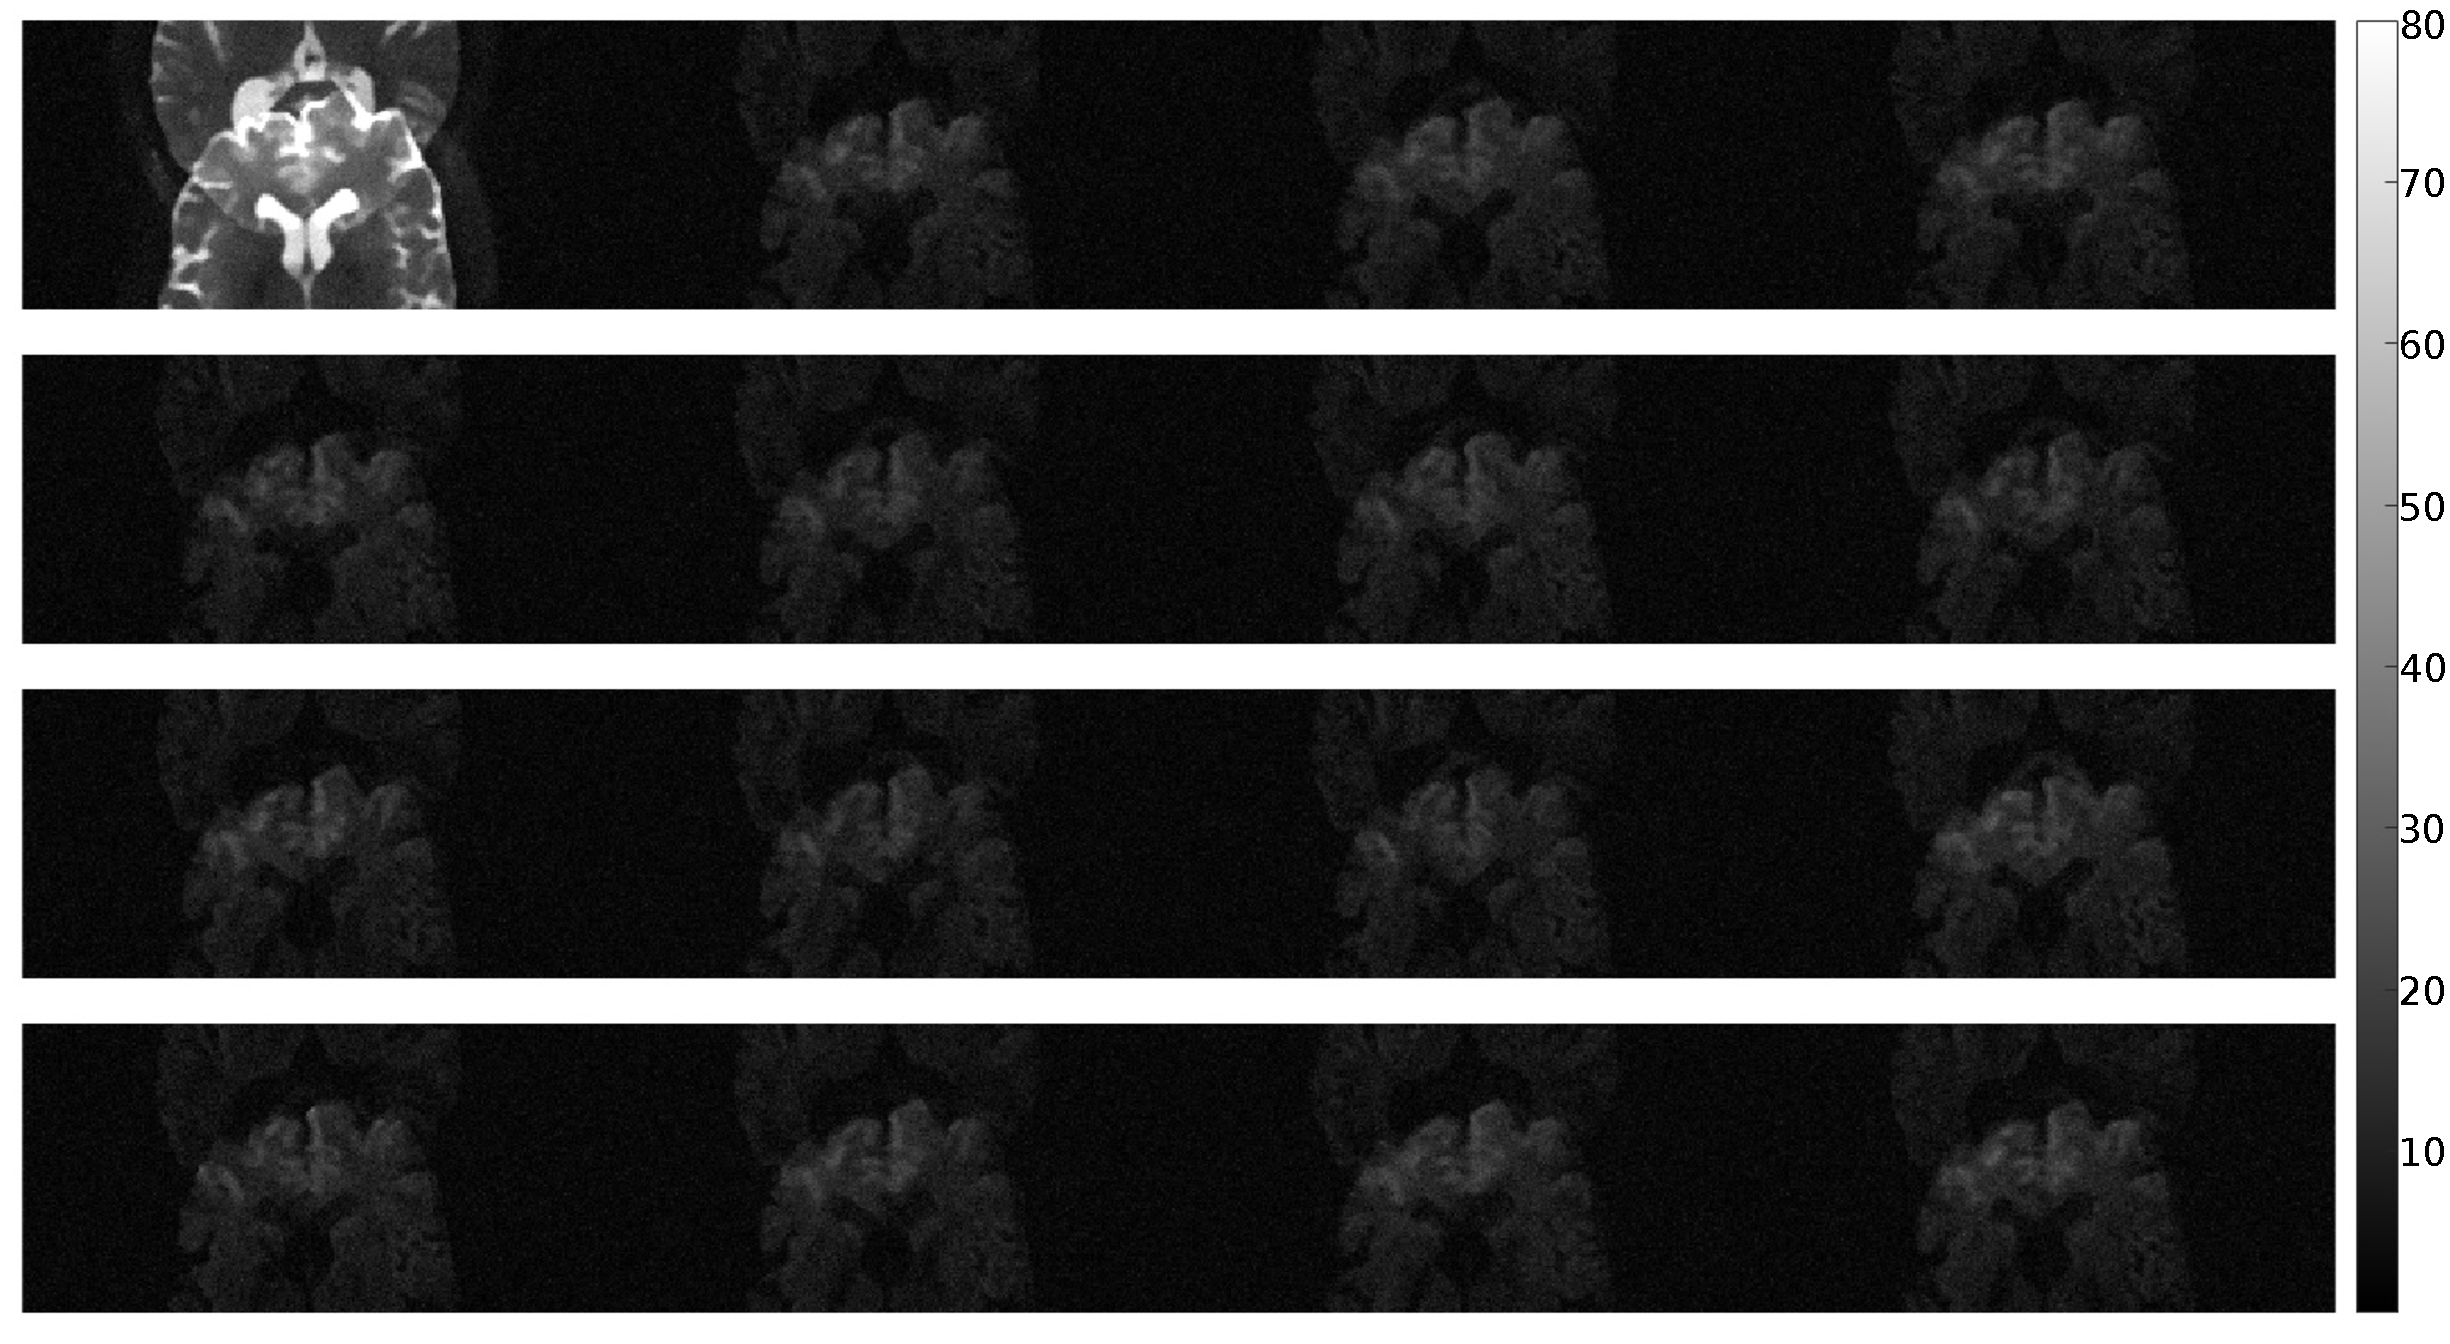
\includegraphics[scale=0.36]{figures/Module_01/NON_RECON.pdf}
  \caption{Subsampled diffusion dataset in \textbf{x}-space domain (data for one particular slice, acquired for 15 diffusion weightening gradients).}
  \label{rys:subsampled}
\end{figure}

\begin{figure}[h!]
\centering
  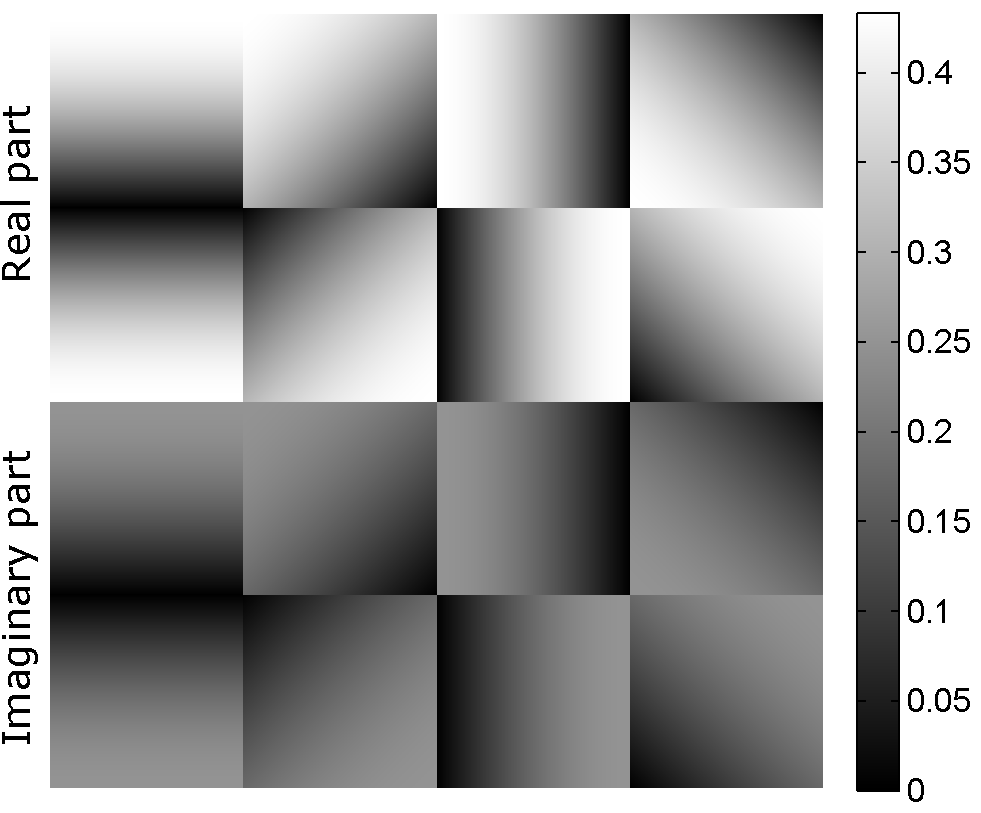
\includegraphics[scale=0.46]{figures/Module_01/MAPS.pdf}
  \caption{The real and imaginary parts of sensitivity maps used to reconstruct data ($L = 8$).}
  \label{rys:maps}
\end{figure}

\begin{figure}[h!]
\centering
  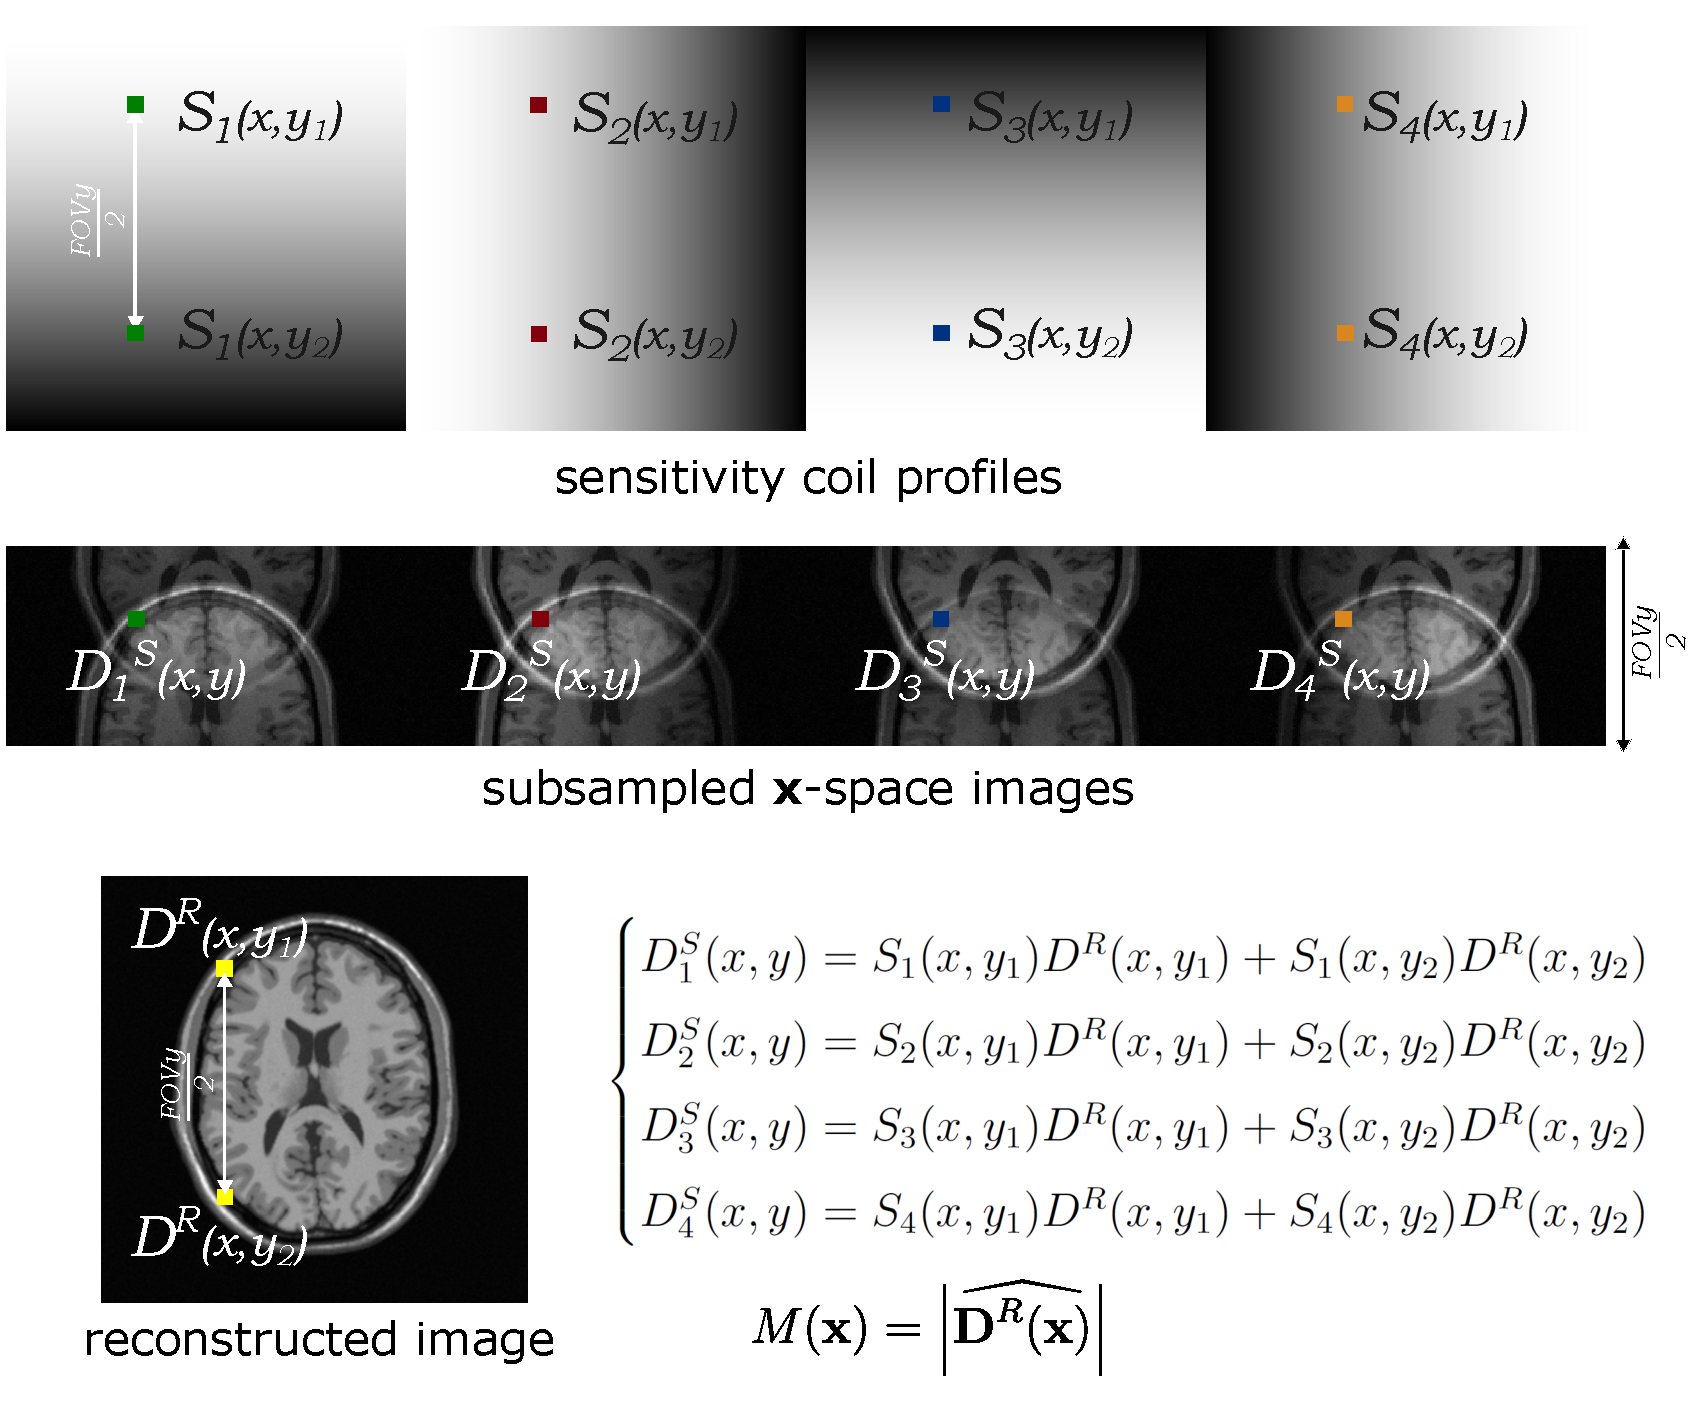
\includegraphics[scale=0.36]{figures/Module_01/SENSE.pdf}
  \caption{SENSE algorithm graphical explanation of Cartesian sampling using four receiver
coils ($L = 4$) and the subsampling rate $r = 2$. Two yellow pixels of the reconstructed image are
unfolded using coil sensitivity profiles and the corresponding folded pixels (points marked with
green, red, blue and orange).}
  \label{rys:sense}
\end{figure}

Thirdly, we used absolute value operator right before performing the SENSE reconstruction main step. As we are provided with sensitivity maps profiles (Fig. \ref{rys:maps}), we can easily reconstruct the subsampled data as it is shown in Fig. \ref{rys:sense}.
The key idea is to evaluate the algorithm pixel by pixel. According to equation \ref{Eq:wzor4}, the construction of defined $\textbf{D}^{S}$ vector is simple. Basically, the $\textbf{D}^{S}$ is a column vector of $L\times1$ size, containing pixels withdrawn from each $L$ coil image at specified spatial location. The matrix $\textbf{S}$ we construct in a~subsequent way: the $l-th$ row of $\textbf{D}^{S}$ contains values of the sensitivity maps profiles, corresponding to data position in a subsampled image and moved by a subsampled FOV value (i.e. for $r=4$, $FOV_{y} = 256/4 = 64$) $r-1$ times. As a result, depending on the number of coils and subsampling rate value, we obtained a matrix of $L\times r$ size. In LSE sense, the result of computation of  for defined $\textbf{D}^{S}$ and~$\textbf{S}$ is column vector $\textbf{D}^{R}$ ($r\times 1$ size). 

However, the LSE approach is not an optimal solution, so we implemented the regularization approach which uses the \textit{a priori} information of searched solution obtained with LSE algorithm. The images obtained after first reconstruction are median filtered with window size$3$x$3$. We introduced this additional information to the solution of derived objective function according to Eq. \ref{Eq:wzor7}. In this case, $\textbf{D}^{S}$ and~$\textbf{S}$ are constructed in the same manner as for LSE case, however we regularized the solution with $\lambda$ parameter. The choice of appropriate value of regularization parameter allows controlling the balance between both components (bias-variance tradeoff). For this scenario, we empirically picked $\lambda$ parameter as a constant value. As the reconstruction is performed pointwisely, we introduced extra information about expected result as a vector $\textbf{D}$ of $r$x$1$ size, containing pixels from reconstructed median filtered LSE images corresponding spatially to those to be reestimated with Tikhonov approach. The result is similar, i.e., we derived values of $r$ reconstructed points, which differ from those obtained with basic LSE approach. Fig. \ref{rys:recon} presents exemplary result of Tikhonov reconstruction algorithm implemented in the software. 

\begin{figure}[h!]
\centering
  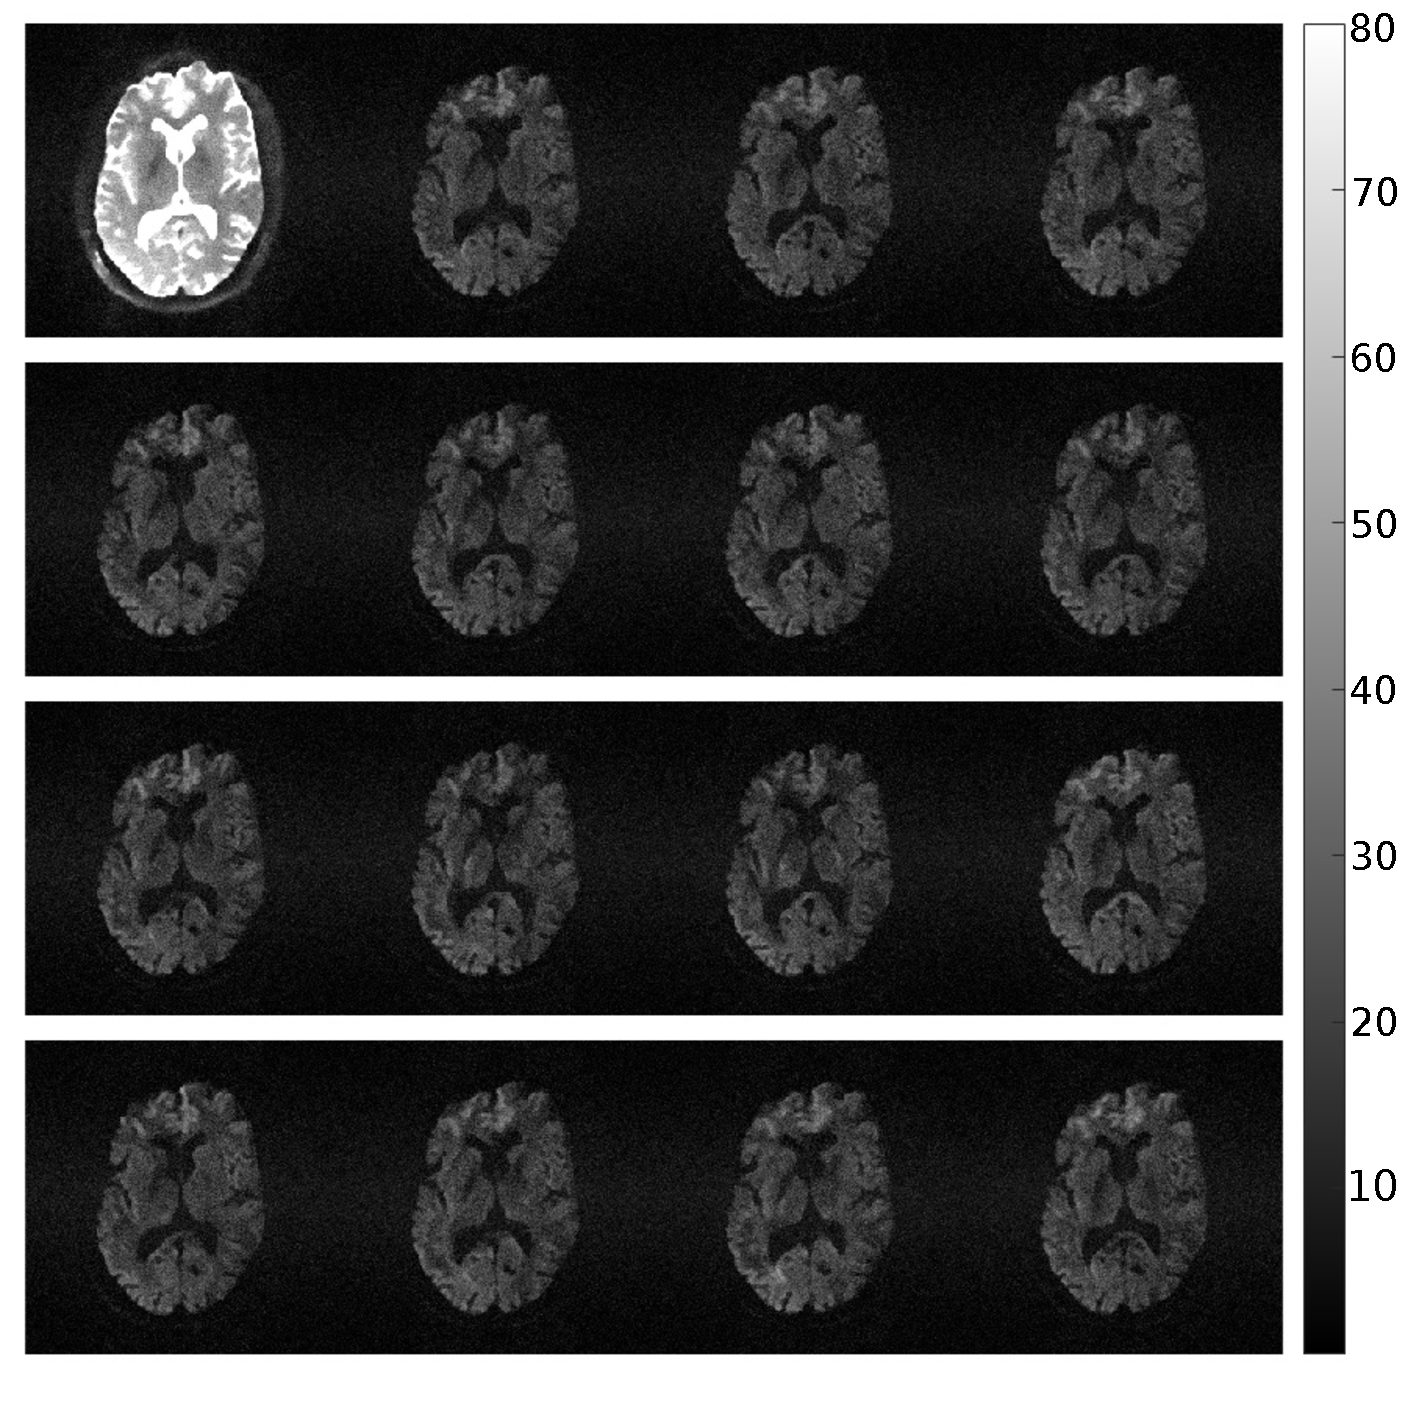
\includegraphics[scale=0.36]{figures/Module_01/RECON.pdf}
  \caption{Reconstructed diffusion dataset in \textbf{x}-space domain (data for one particular slice, acquired for 15 diffusion weightening gradients).}
  \label{rys:recon}
\end{figure}

